% ============================================================
% ARTIGO PRINCIPAL - ARQUIVO ÚNICO
% Indicações Geográficas e Desenvolvimento Territorial no Brasil
% Autores: Ariana Oliveira Gusmão, Wellington Gubiani Maiberg,
%          Hilton Manoel Dias Ribeiro
% Disciplina: Desenvolvimento Regional e Territorial (DRTP)
% ============================================================

\documentclass[12pt, a4paper]{article}

% --- Codificação e idioma ---
\usepackage[utf8]{inputenc}
\usepackage[T1]{fontenc}
\usepackage[brazilian]{babel}

% --- Layout ---
\usepackage[top=3cm, bottom=2cm, left=3cm, right=2cm]{geometry}
\usepackage{setspace}
\onehalfspacing

% --- Matemática ---
\usepackage{amsmath}
\usepackage{amssymb}

% --- Tabelas ---
\usepackage{booktabs}
\usepackage{threeparttable}
\usepackage{multirow}

% --- Figuras ---
\usepackage{graphicx}
\usepackage{float}

% --- Referências ---
\usepackage{natbib}
\bibliographystyle{apalike}

% --- Outros ---
\usepackage{indentfirst}
\usepackage{caption}
\usepackage[colorlinks=true, linkcolor=black, citecolor=black, urlcolor=black]{hyperref}

% --- Caminho das figuras ---
\graphicspath{{Figuras_Artigo/}}

% ============================================================
\begin{document}
% ============================================================

% --- Página de título ---
\begin{titlepage}
\centering
\vspace*{2cm}

{\large Indicações Geográficas e Desenvolvimento Territorial no Brasil: \\[0.4em]
Evidências Causais de Café e Vinho com Propensity Score Matching, \\[0.2em]
Diferenças em Diferenças e \textit{Event Study}}

\vspace{2cm}

{\normalsize
Ariana Oliveira Gusmão \\
Wellington Gubiani Maiberg \\
Hilton Manoel Dias Ribeiro
}

\vspace{1cm}

{\small
Disciplina de Desenvolvimento Regional e Territorial (DRTP)
}

\vfill

{\small Junho de 2026}
\end{titlepage}

% --- Resumo ---
\begin{abstract}
\noindent
As Indicações Geográficas (IGs) são instrumentos de política de desenvolvimento territorial amplamente adotados no Brasil, com 169 registros reconhecidos pelo Instituto Nacional da Propriedade Industrial (INPI). Apesar do crescimento expressivo, a evidência causal sobre seus efeitos em municípios brasileiros ainda é escassa. Este estudo estima e compara o efeito causal do registro de IGs sobre o desenvolvimento municipal nas cadeias produtivas do café e do vinho, combinando \textit{Propensity Score Matching} (PSM), Diferenças em Diferenças (DiD) com efeitos fixos e \textit{Event Study} para um painel de municípios brasileiros entre 2013 e 2023. A combinação dos três métodos permite estimar o efeito médio do tratamento e testar formalmente o pressuposto de tendências paralelas, necessário para interpretação causal. Para o café, o teste revela violação desse pressuposto (coeficiente em $t{-}2$: $-$0,031; p $<$ 0,001) e nenhuma das oito especificações do PSM produz efeito significativo, indicando ausência de efeito causal. Para o vinho, as tendências paralelas são válidas (coeficiente em $t{-}2$: $-$0,001; p $=$ 0,907) e o DiD identifica efeito positivo e significativo sobre o IFDM Emprego e Renda ($+$0,027; p $=$ 0,006). Os resultados sugerem que o impacto das IGs sobre o desenvolvimento territorial é condicional às características da cadeia produtiva, sendo mais pronunciado em produtos intensivos em trabalho e com potencial para encadeamentos locais.

\bigskip
\noindent \textbf{Palavras-chave:} Indicações Geográficas; Desenvolvimento Territorial; Propensity Score Matching; Diferenças em Diferenças; IFDM; Brasil.
\end{abstract}

\newpage
\tableofcontents
\newpage

% ============================================================
\section{Introdução}
% ============================================================

As Indicações Geográficas (IGs) são sinais distintivos que têm por objetivo realizar a distinção de produtos e serviços baseados em sua origem geográfica, indicando com clareza sua proveniência. Esta identidade comum permite fortalecer a imagem da região e valorizar a qualidade de produtos e serviços \citep{inpi2026}. No Brasil, as IGs são protegidas de duas maneiras: Indicação de Procedência (IP), que protege o nome geográfico que se tornou conhecido pela produção de determinado produto ou prestação de serviço, e Denominação de Origem (DO), pela qual se busca conhecer como o produto e o território se relacionam, cujas características de qualidade sejam exclusivamente definidas pelo local de origem \citep{barbosa2010}. As IGs são de suma importância e contribuem para a melhora dos indicadores socioeconômicos locais, promovendo a identificação e a sinalização da origem de determinado produto ou serviço, atrelando-os às características e qualidades regionais \citep{artencio2019}. Seu uso é exclusivo aos produtores e prestadores de serviço estabelecidos no local, exigindo-se ainda, em relação às denominações de origem, o atendimento de requisitos de qualidade \citep{brasil1996}. Desde o registro pioneiro da IG Vale dos Vinhedos, em 2002, o número de IGs brasileiras cresceu de forma expressiva, alcançando atualmente 127 IP e 42 DO reconhecidas pelo Instituto Nacional da Propriedade Industrial (INPI), distribuídas em diferentes regiões do país e abrangendo setores produtivos heterogêneos (de vinhos e café a mármores, artesanato e produtos quilombolas) \citep{inpi2026}. Esse crescimento tem sido acompanhado por um debate crescente sobre os efeitos reais das IGs sobre o desenvolvimento dos territórios onde estão inseridas.

A literatura internacional evidencia que as IGs podem gerar efeitos positivos sobre emprego, renda, exportações e bem-estar das populações locais \citep{medeiros2021raiher, belletti2017}. Contudo, esses efeitos não são automáticos nem uniformes: estudos como o de \citet{vaquero2021} sugerem que dependem das condições territoriais preexistentes, da qualidade do arranjo institucional e da capacidade de cooperação entre os atores locais \citep{maiorki2015}. Regiões com maior vulnerabilidade socioeconômica e baixo capital social tendem a encontrar mais dificuldades em converter o registro da IG em desenvolvimento de fato, ao passo que territórios com arranjos institucionais consolidados e produtores organizados coletivamente apresentam resultados mais expressivos.

Apesar da relevância do tema, estudos que quantifiquem empiricamente os efeitos das IGs sobre o desenvolvimento regional no Brasil ainda são escassos. \citet{medeiros2021raiher} representam um avanço importante ao aplicarem o método \textit{Propensity Score Matching} (PSM) para avaliar os efeitos das IGs de café e vinho em municípios brasileiros, identificando efeitos positivos associados ao registro. O PSM em corte transversal, contudo, compara municípios certificados e não certificados em um único momento no tempo, permitindo estimar uma associação, mas não observa a trajetória dos territórios antes e depois do registro, nem verifica se os municípios que obtiveram IG já se encontravam em rota distinta dos demais antes mesmo da certificação. O presente trabalho retoma a análise dos mesmos dois produtos, o café e o vinho, mas incorpora a dimensão temporal ausente no estudo de \citet{medeiros2021raiher}. Nesse sentido, formula-se a seguinte pergunta de pesquisa: o registro de uma Indicação Geográfica, por si só, gera efeitos econômicos mensuráveis nos municípios brasileiros, ou esses efeitos variam conforme o produto considerado, sugerindo que o grau de organização e de articulação coletiva da cadeia produtiva pode condicionar os resultados, como indicam as diferenças observadas entre o café e o vinho?

Diante disso, o presente estudo tem como objetivo estimar e comparar o efeito causal do registro das IGs sobre o desenvolvimento municipal nas cadeias produtivas do café e do vinho no Brasil, por meio da combinação do PSM, DiD e \textit{Event Study}.

% ============================================================
\section{Revisão da Literatura}
% ============================================================

A relação entre IG e desenvolvimento regional tem sido tema crescente de investigação em literaturas de economia regional, agronegócio, geografia e direito da propriedade intelectual. O debate parte de um questionamento central: as IGs são instrumentos com potencial reconhecido para geração de valor, mas os efeitos observados variam entre produtos, regiões e arranjos institucionais. Esta seção reúne os principais argumentos teóricos e evidências empíricas sobre essa relação, com foco nos trabalhos aplicados que guiam o presente estudo.

Sendo um ativo da propriedade industrial, a IG identifica e protege produtos cujas qualidades únicas estão vinculadas especificamente a uma área geográfica. Seu registro reconhece reputação, qualidade e características atreladas ao local de origem, agregando valor a produtos tradicionais de diversas regiões e protegendo as características do território e o saber-fazer \citep{meggiolaro2020, rangel2023}. As IGs são utilizadas para proteção de produtos industriais e agrícolas e, nas legislações de alguns países, como o Brasil, também para artesanato e serviços, podendo, por meio de tratados internacionais, ter sua proteção solicitada em outros países \citep{ompi2022}.

No Brasil, a IG está classificada em dois tipos: Indicação de Procedência (IP) e Denominação de Origem (DO). De acordo com a Lei n\textsuperscript{o} 9.279, de 14 de maio de 1996, a IP reconhece o nome geográfico que se tornou conhecido como centro de produção de determinado produto; já a DO exige que as qualidades do produto decorram de maneira exclusiva ou essencialmente do meio geográfico, incluídos fatores naturais e humanos \citep{brasil1996}. Essa distinção não é meramente jurídica: ela implica diferentes intensidades de cooperação entre os produtores, diferentes exigências de padronização e diferentes graus de convergência territorial, com consequências diretas sobre os efeitos econômicos. A Organização Mundial da Propriedade Intelectual reconhece as IGs como instrumentos de proteção de produtos locais e valorização do patrimônio cultural dos territórios, reforçando sua dimensão coletiva e pública \citep{ompi2022}.

\citet{belletti2017} apresentam um dos principais referenciais teóricos sobre IG e desenvolvimento sustentável. Para os autores, os efeitos de uma IG não são automáticos e dependem da articulação entre três elementos: viabilidade econômica das empresas da cadeia produtiva, ação coletiva para promoção e controle de qualidade, e preservação dos recursos territoriais que dão identidade ao produto. Quando esses elementos funcionam de forma coordenada, a IG promove diferenciação de mercado e agregação de valor; quando há falhas de governança ou baixa cooperação, seus efeitos tornam-se limitados ou inexistentes. Essa especificidade é o ponto teórico que estrutura a comparação proposta neste estudo entre as cadeias do café e do vinho.

A dimensão econômica das IGs em escala global pode ser ilustrada pelos dados da Comissão Europeia \citeyear{european2020}: em 2017, os produtos com IG nos países da União Europeia geraram valor de vendas estimado em 74,76 bilhões de euros, sendo os vinhos responsáveis por mais da metade (39 bilhões de euros), seguidos pelos produtos agrícolas e alimentos (35\%) e pelas bebidas espirituosas (13\%). O estudo verificou ainda que esses produtos são comercializados, em média, a 2,07 vezes o preço de produtos comparáveis sem certificação, com destaque para os vinhos (2,85) e as bebidas espirituosas (2,52). As exportações de produtos com IG alcançaram 32,10 bilhões de euros em 2017, concentradas em cinco países: França, Itália, Alemanha, Reino Unido e Espanha \citep{european2020}.

No campo empírico, a evidência quantitativa internacional é predominantemente europeia e, em geral, favorável. \citet{cei2018} avaliam o impacto das IGs sobre o desenvolvimento rural em regiões italianas ao nível NUTS3, utilizando dados em painel e abordagem de avaliação de políticas públicas, e encontram impacto positivo direto sobre o valor agregado agrícola regional. \citet{crescenzi2022} e \citet{crescenzi2023} identificam, para o caso europeu, efeitos positivos das IGs sobre o desenvolvimento local e sobre a atração de investimentos, com destaque para o papel do enraizamento territorial. \citet{desimone2024} representam o estado da arte metodológico desse conjunto: combinam o PSM com DiD e um PSM generalizado para captar o efeito do adensamento de certificações, encontrando impacto positivo das IGs de vinho sobre a demanda turística e submetendo as estimativas a testes de tendências paralelas e controles de placebo. Cabe destacar que esses trabalhos mobilizam, isolada ou combinadamente, o PSM e o DiD, e que os estudos mais robustos verificam explicitamente o pressuposto de identificação, delimitando com precisão o ponto em que esta pesquisa avança.

No Brasil, a evidência é mais escassa e majoritariamente qualitativa. \citet{maiorki2015}, a partir de dois casos do setor vinícola do sul do Brasil, concluíram que os efeitos econômicos da IG sobre o território tendem a ser predominantemente indiretos, mediados pelo turismo e pela visibilidade dos produtos certificados sobre os demais itens da cadeia produtiva local. Os autores observaram ainda que a IG, por si só, não é suficiente para promover o desenvolvimento territorial, dependendo da articulação com outros vetores econômicos e da mobilização dos atores locais em torno de objetivos coletivos. O principal estudo quantitativo é o de \citet{medeiros2021raiher}, que aplicam o PSM aos casos do café e do vinho e identificam efeitos positivos associados ao registro, resultado que será reexaminado quando incorporada a dimensão temporal que o corte transversal do PSM não pode captar.

A lacuna que esta pesquisa preenche organiza-se em três dimensões: a ausência de uma aplicação conjunta dos três métodos (PSM, DiD e \textit{Event Study}) ao caso brasileiro; a ausência de uma comparação sistemática entre dois produtos de cadeias produtivas distintas; e o emprego do teste de tendências paralelas não como mera validação de um efeito esperado, mas como instrumento de diagnóstico, capaz de distinguir um efeito causal de um padrão de seleção preexistente.

\subsection{Estratégia de Busca e Seleção da Literatura}
\label{sec:prisma}

Para fundamentar teórica e empiricamente a relação entre IGs e desenvolvimento regional, realizou-se uma revisão sistematizada da literatura conduzida segundo as etapas do protocolo PRISMA (\textit{Preferred Reporting Items for Systematic Reviews and Meta-Analyses}), com o objetivo de mapear a evidência existente sobre os efeitos das IGs no desenvolvimento econômico e territorial e, em especial, de identificar estratégias empíricas já empregadas para estimar esses efeitos.

A busca foi realizada entre maio e junho de 2026 nas bases Scopus e Web of Science (Coleção Principal). A estratégia de busca utilizou termos em inglês como \textit{Geographical Indication}, \textit{Regional Development}, \textit{Innovation} e \textit{Territorial Development} e seus correspondentes, combinados por operadores booleanos (AND e OR) e estratégias de truncagem. Foram considerados artigos e \textit{reviews} publicados entre 2000 e 2026 nos idiomas inglês, português, espanhol e italiano. O gerenciamento das referências foi realizado no software Zotero e a triagem na plataforma Rayyan, com leitura dos títulos, resumos e palavras-chave à luz de critérios de elegibilidade previamente definidos: estudos empíricos que medissem os efeitos das IGs sobre dimensões de desenvolvimento, excluindo-se textos exclusivamente jurídicos ou normativos, estudos sem mensuração de efeito e trabalhos sem aderência ao objetivo.

A busca resultou em 1.976 registros (1.029 na Scopus e 947 na Web of Science). Após a remoção de 738 duplicatas, permaneceram 1.238 registros únicos. Desse conjunto, 885 foram excluídos por não aderência aos critérios e 353 retidos para análise (284 incluídos e 69 reservados para nova triagem). A Tabela~\ref{tab:prisma_etapas} resume as etapas do processo.

\begin{table}[htbp]
\centering
\caption{Etapas de desenvolvimento da revisão de literatura}
\label{tab:prisma_etapas}
\begin{threeparttable}
\begin{tabular}{ll}
\toprule
\textbf{Etapa} & \textbf{Procedimento} \\
\midrule
Busca         & Scopus e Web of Science \\
Gerenciamento & Organização das referências no Zotero \\
Tratamento    & Remoção de registros duplicados \\
Triagem       & Leitura de títulos, resumos e palavras-chave \\
Seleção       & Leitura integral dos artigos aderentes \\
Análise       & Classificação temática e análise de conteúdo \\
\bottomrule
\end{tabular}
\begin{tablenotes}
\small
\item Fonte: Os autores (2026).
\end{tablenotes}
\end{threeparttable}
\end{table}

% ============================================================
\section{Dados}
% ============================================================

\subsection{Fontes}

Este estudo combina quatro bases de dados públicas para o período de 2013 a 2023.

O indicador de desenvolvimento municipal utilizado é o \textbf{Índice FIRJAN de Desenvolvimento Municipal (IFDM)} \citep{firjan2023}, elaborado pela Federação das Indústrias do Rio de Janeiro com base em registros administrativos do governo federal. O índice varia de 0 a 1 e é decomposto em três dimensões: Emprego e Renda (baseado na RAIS), Educação (Censo Escolar) e Saúde (SINASC e SIM). Utilizamos o IFDM Geral e os três subíndices como variáveis de resultado.

Os dados sobre \textbf{Produto Interno Bruto (PIB) municipal e Valor Adicionado setorial} provêm das Contas Regionais do IBGE \citep{ibge2023}, disponíveis anualmente por município. Para exportações, utilizamos os microdados do \textbf{ComexStat/MDIC} \citep{comexstat2024}, filtrando os produtos da posição SH4 0901 (café, mesmo torrado ou descafeinado), agregados por município exportador e ano.

As \textbf{Indicações Geográficas (IGs)} foram obtidas de duas fontes complementares: o banco de dados do MAPA \citep{mapa2023} (Ministério da Agricultura), que lista os municípios abrangidos por cada IG, e o INPI \citep{inpi2026} (Instituto Nacional da Propriedade Industrial), que registra o ano de concessão de cada IG. A combinação dessas fontes permitiu identificar, para cada município tratado, o ano exato em que a IG foi reconhecida, informação essencial para o \textit{design} de tratamento escalonado adotado neste estudo.

A Figura~\ref{fig:mapa} apresenta a distribuição geográfica dos municípios tratados no Brasil.

\begin{figure}[htbp]
\centering
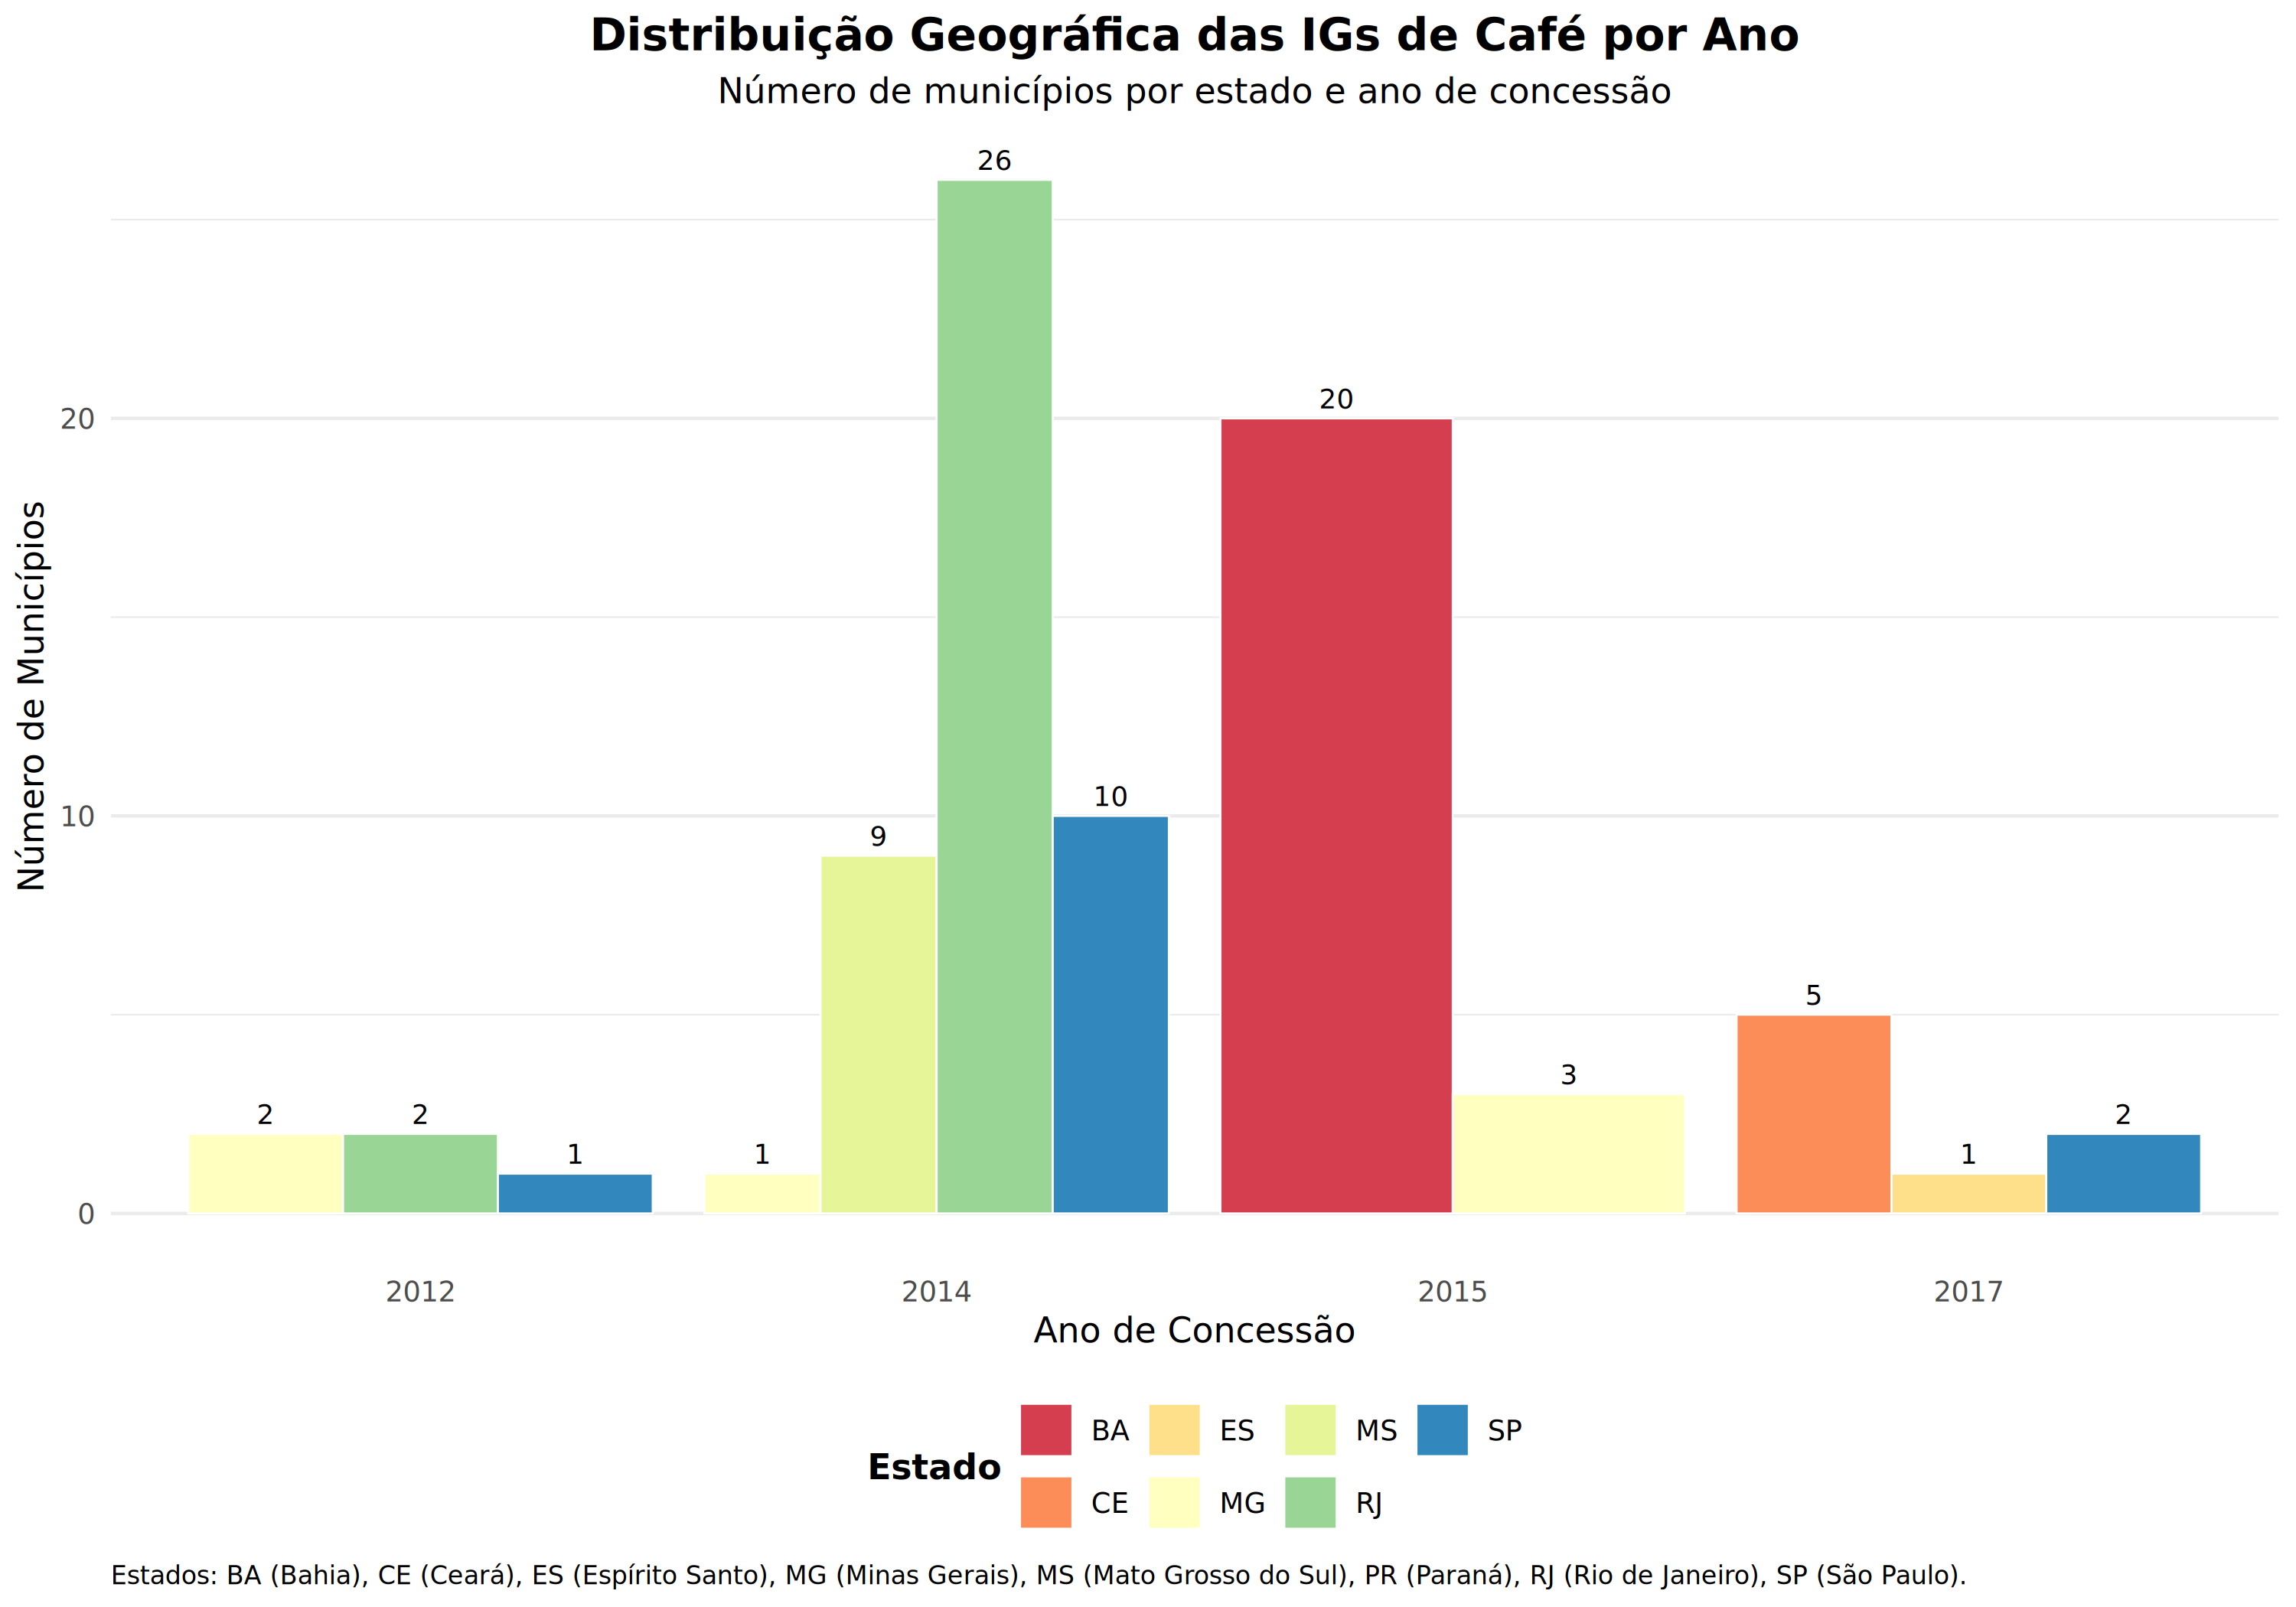
\includegraphics[width=0.82\textwidth]{Distribuicao_Geografica_IGs.png}
\caption{Distribuição geográfica dos municípios com Indicação Geográfica}
\label{fig:mapa}
\begin{minipage}{0.85\textwidth}
\small \textit{Nota:} Municípios identificados via MAPA e INPI. Café concentrado no Sudeste e Nordeste; vinho concentrado no Sul e no Vale do São Francisco.
\end{minipage}
\end{figure}

\subsection{Amostra de café}

A partir do cadastro do MAPA, identificamos 87 municípios brasileiros abrangidos por pelo menos uma das 24 IGs de café registradas até 2017. Desses, 83 foram pareados com sucesso na etapa de \textit{matching} (Seção~\ref{sec:psm}), conformando o grupo tratado.

Das 87 com IG identificada, 86 têm ano de concessão confirmado, distribuídas em quatro coortes: 2012 (5 municípios), 2014 (50 municípios), 2015 (23 municípios) e 2017 (8 municípios). A maioria, correspondente a 58\% dos municípios com ano de concessão conhecido, recebeu a IG em 2014, em função de um processo coletivo de reconhecimento em diversas regiões do Brasil naquele ano. Os municípios tratados estão distribuídos principalmente nos estados de Minas Gerais, Espírito Santo, Rio de Janeiro e Bahia, abrangendo regiões produtoras como o Cerrado Mineiro, a Chapada Diamantina e a região de Machado.

\subsection{Amostra de vinho}

Para o vinho, identificamos 31 municípios tratados a partir de seis IGs com concessão anterior a 2017, condição necessária para observar ao menos seis anos de pós-tratamento no painel disponível. A Tabela~\ref{tab:igs_vinho} lista as IGs utilizadas.

\begin{table}[htbp]
\centering
\caption{IGs de vinho incluídas na análise}
\label{tab:igs_vinho}
\begin{threeparttable}
\begin{tabular}{lccc}
\toprule
Indicação Geográfica & Ano & UF & N Municípios \\
\midrule
Vale dos Vinhedos (IP) & 2002 & RS    & 3 \\
Vales da Uva Goethe    & 2012 & SC    & 6 \\
Vale do São Francisco  & 2014 & PE/BA & 5 \\
Altos Montes           & 2015 & RS    & 2 \\
Campanha Gaúcha        & 2015 & RS    & 14 \\
Farroupilha            & 2015 & RS    & 1 \\
\midrule
\textbf{Total} & & & \textbf{31} \\
\bottomrule
\end{tabular}
\begin{tablenotes}
\small
\item Fonte: INPI e MAPA. Inclui apenas IGs com concessão $\leq$ 2017.
\end{tablenotes}
\end{threeparttable}
\end{table}

A vinicultura brasileira está concentrada geograficamente, com forte presença no Rio Grande do Sul (20 dos 31 municípios), o que contrasta com a dispersão geográfica das IGs de café.

\subsection{Estatísticas descritivas}

A Tabela~\ref{tab:descritivas} apresenta as características médias dos municípios tratados (café) e do conjunto de municípios sem IG, observadas em 2013, ano anterior ao principal bloco de concessões e utilizado como linha de base.

\begin{table}[htbp]
\centering
\caption{Características pré-tratamento dos municípios (2013)}
\label{tab:descritivas}
\begin{threeparttable}
\begin{tabular}{lccc}
\toprule
Variável & Café c/ IG (n=87) & Sem IG (n$\approx$5.483) & Diferença \\
\midrule
IFDM Geral                        & 0,602 & 0,582 & $+$0,020$^{**}$ \\
IFDM Emprego e Renda              & 0,496 & 0,478 & $+$0,018$^{*}$  \\
IFDM Educação                     & 0,660 & 0,648 & $+$0,012        \\
IFDM Saúde                        & 0,649 & 0,620 & $+$0,029$^{**}$ \\
PIB \textit{per capita} (R\$ mil) & 18,3  & 16,7  & $+$1,6          \\
População (mil)                   & 35,2  & 33,8  & $+$1,4          \\
\bottomrule
\end{tabular}
\begin{tablenotes}
\small
\item Fonte: FIRJAN (IFDM) e IBGE (PIB, População).
\item $^{**}$ p $<$ 0,05;\; $^{*}$ p $<$ 0,10.
\end{tablenotes}
\end{threeparttable}
\end{table}

Os municípios com IG de café apresentam IFDM sistematicamente superior ao dos demais municípios antes do recebimento da certificação, o que evidencia \textbf{viés de seleção}: municípios mais desenvolvidos tendem a organizar IGs com mais facilidade. Isso reforça a necessidade de métodos que controlem essa diferença de partida, como o PSM e o DiD com efeitos fixos, descritos a seguir.

% ============================================================
\section{Metodologia}
% ============================================================

Este estudo emprega três métodos complementares para estimar o efeito causal das IGs: \textit{Propensity Score Matching} (PSM), Diferenças em Diferenças (DiD) com efeitos fixos e \textit{Event Study}. A combinação dos três permite não apenas estimar o efeito médio do tratamento, mas também testar se os pressupostos necessários para identificação causal são atendidos.

\subsection{Propensity Score Matching (PSM)}
\label{sec:psm}

O problema fundamental na estimação do efeito das IGs é que os municípios que as recebem não são escolhidos aleatoriamente: tendem a ser mais desenvolvidos, mais organizados institucionalmente e com perfil produtivo diferente. Comparar diretamente municípios com e sem IG produziria estimativas enviesadas.

O PSM resolve isso construindo um grupo de comparação de municípios sem IG que sejam similares aos municípios tratados em todas as características observáveis relevantes \citep{rosenbaum1983, caliendo2008}. Para cada município, estimamos a probabilidade de ter recebido uma IG (o \textit{propensity score}) por meio de uma regressão logística sobre características observadas em 2013:

\begin{align*}
\text{Café:} \quad  & P(\text{IG}=1) \sim \text{PIB}_{pc} + \text{VA}_{agro} + \text{VA}_{ind} + \text{VA}_{serv} \\
                    & \quad + \text{Part}_{agro} + \text{IFDM}_{edu} + \text{IFDM}_{sau} \\[4pt]
\text{Vinho:} \quad & P(\text{IG}=1) \sim \text{IFDM}_{geral} + \text{IFDM}_{edu} + \text{IFDM}_{sau} + \text{IFDM}_{emp}
\end{align*}

Cada município tratado é então pareado com até três municípios de controle cujo \textit{propensity score} seja o mais próximo (\textit{Nearest Neighbor} 3:1, com reposição). Impusemos um \textit{caliper} (distância máxima tolerada entre os \textit{propensity scores} pareados) de 0,01 para café e 0,05 para vinho. O efeito médio do tratamento sobre os tratados (ATT) é estimado por regressão ponderada com erros padrão robustos de Abadie-Imbens.

A qualidade do pareamento é verificada pela diferença padronizada entre os grupos. A Tabela~\ref{tab:balanceamento} mostra que, após o pareamento para café, todas as diferenças padronizadas ficaram abaixo de 0,025, valor muito inferior ao limiar convencional de 0,10, indicando excelente balanceamento. A Figura~\ref{fig:loveplot} apresenta o \textit{Love Plot} correspondente.

\begin{table}[htbp]
\centering
\caption{Balanceamento pós-\textit{matching}: Café}
\label{tab:balanceamento}
\footnotesize
\begin{threeparttable}
\begin{tabular}{lcccc}
\toprule
Variável & Tratados (n=83) & Controles (n=237) & Dif.\ Padronizada & p-valor \\
\midrule
IFDM Geral 2013                        & 0,603 & 0,601 & 0,018 & 0,854 \\
IFDM Emprego e Renda 2013              & 0,497 & 0,495 & 0,019 & 0,843 \\
IFDM Educação 2013                     & 0,661 & 0,658 & 0,024 & 0,795 \\
IFDM Saúde 2013                        & 0,651 & 0,649 & 0,015 & 0,878 \\
PIB \textit{per capita} 2013 (R\$ mil) & 18,2  & 18,0  & 0,021 & 0,825 \\
\bottomrule
\end{tabular}
\begin{tablenotes}
\small
\item \textit{Nearest Neighbor} 3:1, \textit{caliper} 0,01, com reposição.
\item Todas as diferenças padronizadas $< 0{,}025$.
\end{tablenotes}
\end{threeparttable}
\end{table}

\begin{figure}[htbp]
\centering
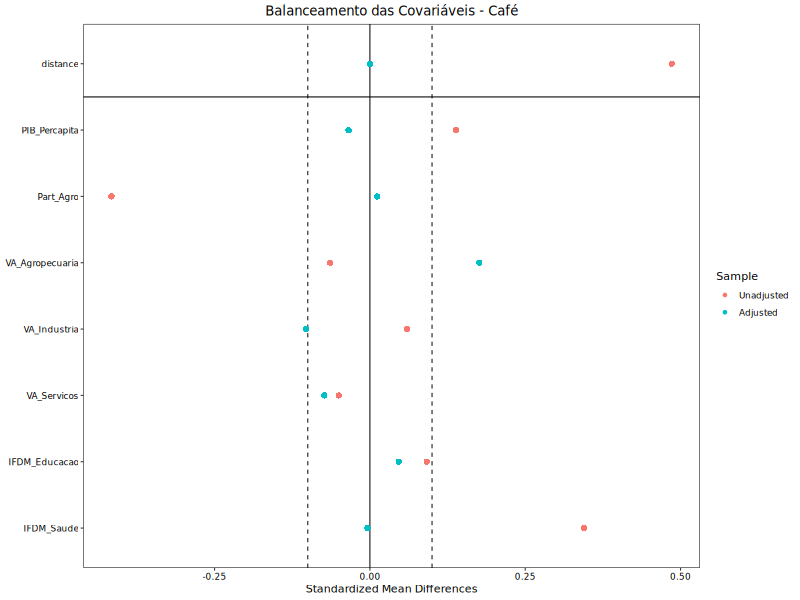
\includegraphics[width=0.82\textwidth]{PSM_Cafe_LovePlot.png}
\caption{\textit{Love Plot}: balanceamento antes e após o \textit{matching} (Café)}
\label{fig:loveplot}
\begin{minipage}{0.85\textwidth}
\small \textit{Nota:} Diferenças padronizadas antes (círculos abertos) e após (círculos preenchidos) o \textit{matching}. Linha vertical em 0,10 indica o limiar convencional de aceitação. Todas as covariáveis ficam abaixo desse limiar após o pareamento.
\end{minipage}
\end{figure}

\subsection{Diferenças em Diferenças com Efeitos Fixos}

Para explorar a dimensão temporal do painel (2013-2023) e controlar por diferenças não observadas permanentes entre municípios, aplicamos o estimador de Diferenças em Diferenças (DiD) com efeitos fixos de dois sentidos (\textit{Two-Way Fixed Effects}, TWFE) \citep{callaway2021, goodmanbacon2021}:

\begin{equation}
Y_{it} = \beta \cdot \text{pos\_trat}_{it} + \alpha_i + \gamma_t + \varepsilon_{it}
\label{eq:did}
\end{equation}

\noindent onde $Y_{it}$ é o IFDM do município $i$ no ano $t$; $\text{pos\_trat}_{it}$ é uma variável binária que vale 1 se o município $i$ possui IG e o ano $t$ é igual ou posterior ao ano de concessão dessa IG; $\alpha_i$ são efeitos fixos de município, que absorvem todas as diferenças permanentes entre municípios; $\gamma_t$ são efeitos fixos de ano, que absorvem choques macroeconômicos comuns a todos os municípios; e $\varepsilon_{it}$ é o termo de erro, com erros padrão clusterizados no nível do município.

O coeficiente $\beta$ captura o efeito médio da IG nos municípios tratados \textbf{após} a concessão, em comparação com a trajetória dos municípios de controle. O \textit{design} de \textbf{tratamento escalonado} respeita o ano exato de concessão de cada IG, ao invés de usar uma data de corte única para todos. A amostra utilizada no DiD é a mesma amostra pareada pelo PSM.

\subsection{Event Study: Teste de Tendências Paralelas}

O pressuposto fundamental do DiD é o de \textbf{tendências paralelas}: na ausência da IG, tratados e controles teriam evoluído de forma semelhante ao longo do tempo. Se municípios que recebem IGs já estiverem em trajetória diferente dos controles antes da concessão, o estimador DiD não identifica um efeito causal.

O \textit{Event Study} permite testar esse pressuposto diretamente. Em vez de estimar um único coeficiente médio, estimam-se coeficientes separados para cada período relativo à concessão da IG:

\begin{equation}
Y_{it} = \sum_{k \neq -1} \beta_k \cdot D_{it}^k + \alpha_i + \gamma_t + \varepsilon_{it}
\label{eq:eventstudy}
\end{equation}

\noindent onde $D_{it}^k = 1$ se o município $i$ está exatamente $k$ anos distante de sua data de concessão no ano $t$. O período $k = -1$ (ano imediatamente anterior à concessão) é omitido como referência.

Os coeficientes \textbf{pré-tratamento} ($k < -1$) constituem o teste de tendências paralelas: se forem estatisticamente iguais a zero, os dois grupos apresentavam trajetórias paralelas antes da IG, validando a identificação causal. Se algum coeficiente pré-tratamento for significativamente diferente de zero, há evidência de que as trajetórias já divergiam antes da política, o que invalida o DiD.

Para o vinho, o \textit{Event Study} é restrito às coortes de 2014 e 2015 (22 municípios), que possuem pelo menos um ano de pré-período dentro do painel 2013-2023. As IGs concedidas em 2002 (Vale dos Vinhedos, 3 municípios) e 2012 (Vales da Uva Goethe, 6 municípios) foram excluídas desse teste por não terem pré-período observável na amostra disponível.

Cabe notar que esses 9 municípios configuram unidades \textbf{sempre tratadas} no painel: como receberam a IG antes de 2013, a variável $\text{pos\_trat}_{it}$ assume valor 1 em todos os anos observados. No estimador TWFE, unidades sem variação temporal no tratamento têm seu efeito inteiramente absorvido pelo efeito fixo municipal ($\alpha_i$), não contribuindo para a identificação do coeficiente $\beta$. O efeito causal estimado pelo DiD é, portanto, identificado pelas coortes de 2014 e 2015, exatamente as mesmas validadas pelo \textit{Event Study}.

\subsection{Análise de Robustez}

Para o café, testamos a sensibilidade dos resultados do PSM a oito especificações alternativas, variando o \textit{caliper} (0,005; 0,01; 0,05), o número de controles por tratado (1:1; 3:1; 5:1), a permissão de reposição e o algoritmo de \textit{matching} (\textit{Kernel} e \textit{Radius}).

% ============================================================
\section{Resultados}
% ============================================================

\subsection{Café: PSM e Efeito no Desenvolvimento Municipal}

A Tabela~\ref{tab:psm_cafe} apresenta os ATTs estimados pelo PSM para os municípios com IG de café. Em nenhuma das quatro dimensões do IFDM o efeito estimado é estatisticamente significativo ao nível de 10\%.

\begin{table}[htbp]
\centering
\caption{Efeito das IGs de café no IFDM (PSM)}
\label{tab:psm_cafe}
\begin{threeparttable}
\begin{tabular}{lcccc}
\toprule
Variável de Resultado & ATT & Erro Padrão & p-valor & IC 95\% \\
\midrule
IFDM Geral           & $+$0,0094 & 0,0164 & 0,565 & [$-$0,023\,;\,$+$0,042] \\
IFDM Emprego e Renda & $+$0,0222 & 0,0269 & 0,411 & [$-$0,031\,;\,$+$0,075] \\
IFDM Educação        & $+$0,0128 & 0,0151 & 0,397 & [$-$0,017\,;\,$+$0,043] \\
IFDM Saúde           & $+$0,0182 & 0,0192 & 0,343 & [$-$0,020\,;\,$+$0,056] \\
\bottomrule
\end{tabular}
\begin{tablenotes}
\small
\item 83 municípios tratados, 237 controles. \textit{Nearest Neighbor} 3:1, \textit{caliper} 0,01, com reposição.
\item Erro padrão robusto Abadie-Imbens.
\end{tablenotes}
\end{threeparttable}
\end{table}

Os efeitos estimados são positivos, porém pequenos, com intervalos de confiança que incluem amplamente o zero. As variáveis econômicas reforçam esse diagnóstico:

\begin{table}[htbp]
\centering
\caption{Efeito das IGs de café nas variáveis econômicas (PSM)}
\label{tab:psm_cafe_econ}
\begin{threeparttable}
\begin{tabular}{lccc}
\toprule
Variável de Resultado & ATT & Erro Padrão & p-valor \\
\midrule
PIB \textit{per capita}         & $-$R\$\,1.119     & R\$\,3.302    & 0,735 \\
Valor Adicionado Agropecuário   & $+$R\$\,18.384    & R\$\,12.321   & 0,137 \\
Exportações de café (US\$)      & $+$US\$\,9,5\,mi  & US\$\,7,9\,mi & 0,238 \\
Preço médio exportado (US\$/kg) & $-$1,12           & 1,46          & 0,440 \\
\bottomrule
\end{tabular}
\begin{tablenotes}
\small
\item Mesma amostra pareada. Exportações: SH4 0901, ComexStat/MDIC.
\end{tablenotes}
\end{threeparttable}
\end{table}

Mesmo o Valor Adicionado Agropecuário, a variável mais diretamente ligada à atividade cafeeira, apresenta magnitude expressiva (+36\% em relação à média dos controles), mas não alcança significância estatística.

\subsection{Café: DiD e Invalidação pelo Event Study}

O DiD com efeitos fixos produz um coeficiente de $+$0,0088 para o IFDM Geral, marginalmente significativo a 10\% (p = 0,081). À primeira vista, esse resultado poderia sugerir um efeito positivo das IGs. Entretanto, o \textit{Event Study} demonstra que esse resultado é \textbf{espúrio}.

A Tabela~\ref{tab:eventstudy_cafe} apresenta os coeficientes por período relativo à concessão, e a Figura~\ref{fig:es_cafe} os ilustra graficamente.

\begin{table}[htbp]
\centering
\caption{\textit{Event Study}: Café, coeficientes por período relativo à concessão}
\label{tab:eventstudy_cafe}
\begin{threeparttable}
\begin{tabular}{lcccc}
\toprule
Período relativo & Coeficiente & Erro Padrão & p-valor & Interpretação \\
\midrule
$t = -4$        & $-$0,0099 & 0,0096 & 0,302   & OK \\
$t = -3$        & $-$0,0144 & 0,0099 & 0,145   & Declínio incipiente \\
$t = -2$        & $\mathbf{-0{,}0315}$ & $\mathbf{0{,}0083}$ & $\mathbf{<0{,}001}$ & \textbf{Violação}$^{***}$ \\
$t = -1$        & 0         & $\cdot$ & $\cdot$ & (referência) \\
$t = 0$         & $-$0,0044 & 0,0054 & 0,411   & $\cdot$ \\
$t = +1$        & $-$0,0035 & 0,0049 & 0,473   & $\cdot$ \\
$t = +2$        & $-$0,0101 & 0,0051 & 0,046   & Negativo$^{*}$ \\
$t = +3$        & $-$0,0043 & 0,0044 & 0,323   & $\cdot$ \\
$t = +4$ a $+6$ & $\approx 0$ & $\cdot$ & $>$0,30 & $\cdot$ \\
\bottomrule
\end{tabular}
\begin{tablenotes}
\small
\item \textit{Two-Way Fixed Effects}. Erros padrão clusterizados por município.
\item $^{***}$ p $<$ 0,01;\; $^{*}$ p $<$ 0,10.
\end{tablenotes}
\end{threeparttable}
\end{table}

O coeficiente em $t = -2$ é $-$0,031 (p $<$ 0,001): \textbf{dois anos antes de receber a IG, os municípios tratados já estavam em declínio relativo}. Isso indica que a concessão da IG não foi exógena, pois municípios em dificuldade econômica teriam buscado a certificação como resposta a esse declínio. O pressuposto de tendências paralelas é violado e o efeito estimado pelo DiD não pode ser interpretado como causal. Trata-se de reversão à média, não de impacto da política.

\begin{figure}[htbp]
\centering
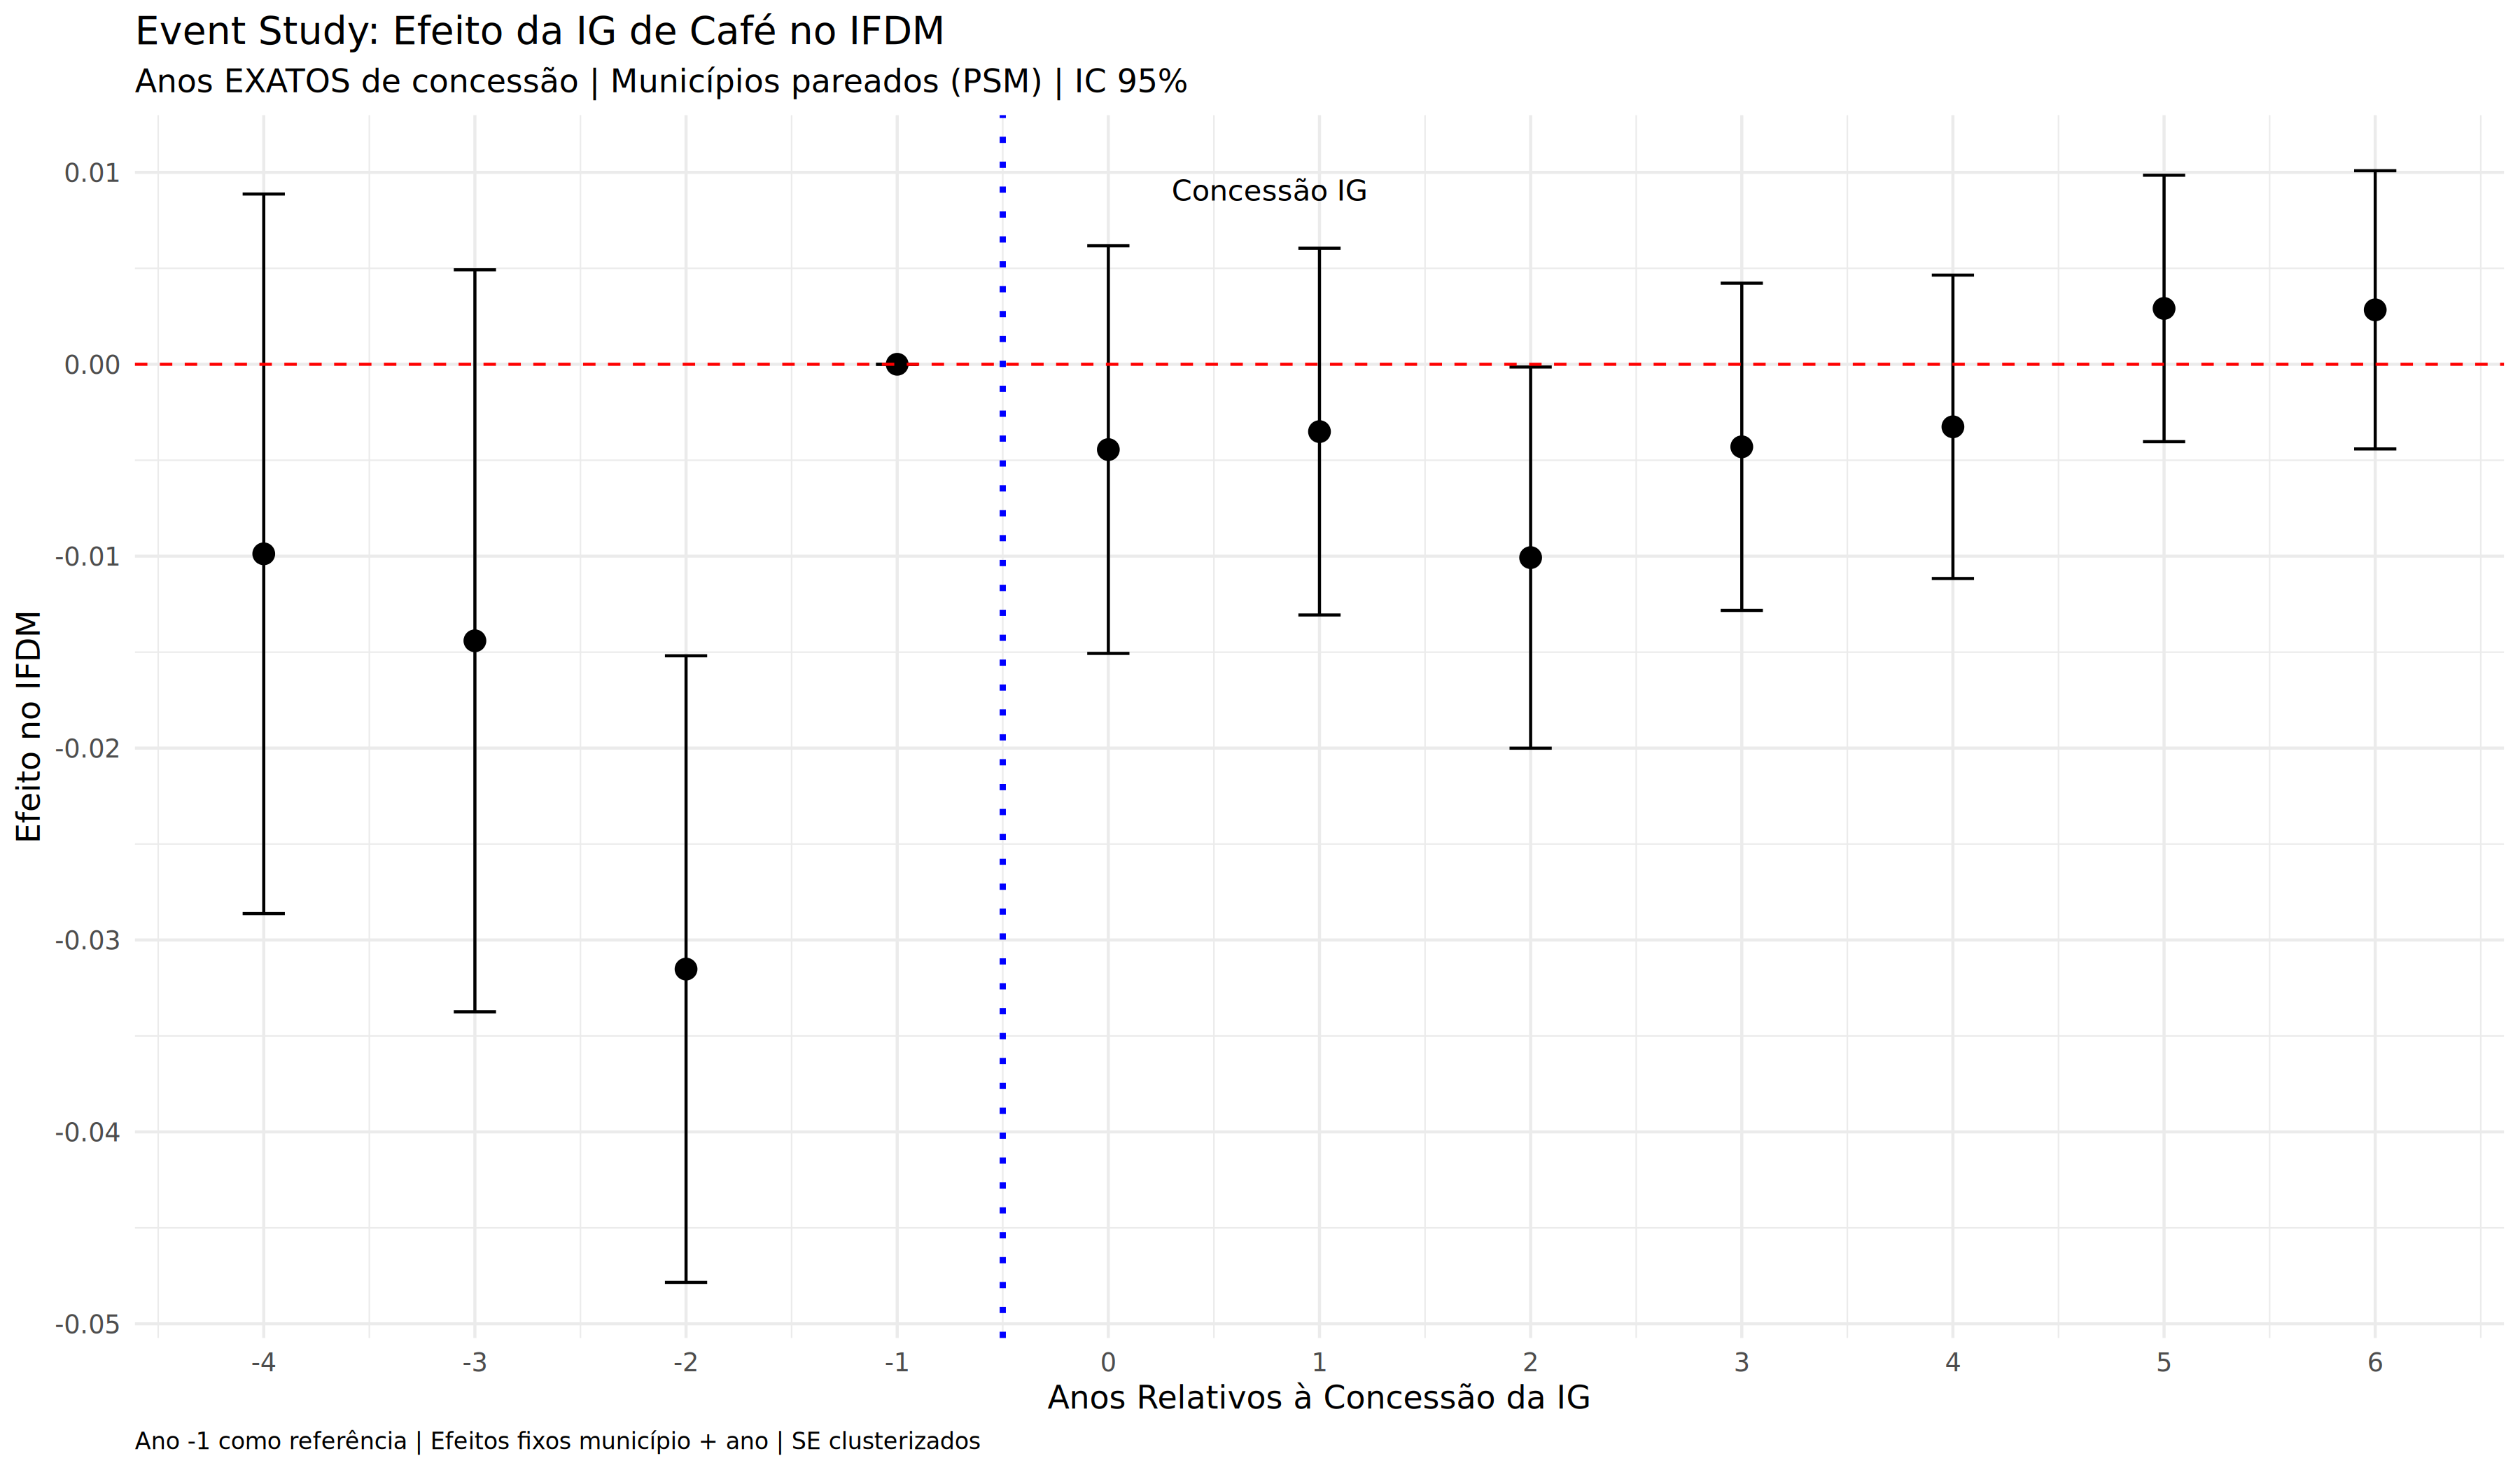
\includegraphics[width=0.82\textwidth]{DiD_EventStudy_AnosExatos.png}
\caption{\textit{Event Study}: Café (IFDM Geral)}
\label{fig:es_cafe}
\begin{minipage}{0.85\textwidth}
\small \textit{Nota:} Coeficientes $\hat{\beta}_k$ estimados pelo TWFE com IC 95\%. O coeficiente em $t = -2$ é significativamente negativo (p $<$ 0,001), evidenciando violação de tendências paralelas. Ano $-1$ omitido como referência.
\end{minipage}
\end{figure}

\subsection{Café: Robustez com 8 Especificações PSM}

A Tabela~\ref{tab:robustez_cafe} apresenta os resultados do PSM para IFDM Geral em oito especificações alternativas.

\begin{table}[htbp]
\centering
\caption{Análise de robustez: PSM com especificações alternativas (Café)}
\label{tab:robustez_cafe}
\begin{threeparttable}
\begin{tabular}{lcccccc}
\toprule
Especificação & \textit{Caliper} & Ratio & Reposição & ATT & Erro Padrão & p-valor \\
\midrule
1. \textit{Baseline}      & 0,01  & 3:1   & Sim & $+$0,0094 & 0,0164 & 0,565 \\
2. \textit{Caliper} menor & 0,005 & 3:1   & Sim & $+$0,0082 & 0,0171 & 0,631 \\
3. \textit{Caliper} maior & 0,05  & 3:1   & Sim & $+$0,0103 & 0,0159 & 0,517 \\
4. Ratio 1:1              & 0,01  & 1:1   & Sim & $+$0,0088 & 0,0176 & 0,617 \\
5. Ratio 5:1              & 0,01  & 5:1   & Sim & $+$0,0097 & 0,0161 & 0,547 \\
6. Sem reposição          & 0,01  & 3:1   & Não & $+$0,0079 & 0,0168 & 0,638 \\
7. \textit{Kernel}        & $\cdot$ & $\cdot$ & $\cdot$ & $+$0,0106 & 0,0153 & 0,489 \\
8. \textit{Radius}        & 0,01  & $\cdot$ & $\cdot$ & $+$0,0091 & 0,0165 & 0,581 \\
\bottomrule
\end{tabular}
\begin{tablenotes}
\small
\item Variável de resultado: IFDM Geral. \textbf{0 de 8 especificações com efeito significativo a 10\%.}
\end{tablenotes}
\end{threeparttable}
\end{table}

Os ATTs variam entre $+$0,0079 e $+$0,0106, sempre com p-valor acima de 0,48. A ausência de efeito é extremamente robusta a diferentes escolhas metodológicas.

\subsection{Vinho: Efeito no Emprego}

Para o vinho, o PSM em corte transversal não produz efeitos significativos nos anos de 2018 e 2022. O DiD com efeitos fixos sobre o painel completo (124 municípios $\times$ 11 anos), porém, revela um padrão distinto. A Tabela~\ref{tab:did_vinho} apresenta os resultados.

\begin{table}[htbp]
\centering
\caption{Efeito das IGs de vinho no IFDM (DiD com Efeitos Fixos)}
\label{tab:did_vinho}
\begin{threeparttable}
\begin{tabular}{lcccc}
\toprule
Variável de Resultado & ATT & Erro Padrão & p-valor & Sig. \\
\midrule
IFDM Geral                    & $+$0,009 & 0,007 & 0,210 & $\cdot$ \\
IFDM Educação                 & $-$0,015 & 0,009 & 0,099 & $^{*}$ (negativo) \\
IFDM Saúde                    & $+$0,016 & 0,016 & 0,335 & $\cdot$ \\
\textbf{IFDM Emprego e Renda} & $\mathbf{+0{,}027}$ & $\mathbf{0{,}010}$ & $\mathbf{0{,}006}$ & $^{***}$ \\
\bottomrule
\end{tabular}
\begin{tablenotes}
\small
\item 31 municípios tratados, 93 controles (PSM \textit{caliper} 0,05, NN 3:1).
\item \textit{Two-Way Fixed Effects}. Erros padrão clusterizados por município.
\item $^{***}$ p $<$ 0,01;\; $^{*}$ p $<$ 0,10.
\end{tablenotes}
\end{threeparttable}
\end{table}

O IFDM Emprego e Renda apresenta efeito de $+$0,027 (p = 0,006), significativo ao nível de 1\%. Esse valor equivale a aproximadamente \textbf{3,9\% acima da média dos municípios de controle}, um efeito economicamente relevante. As demais dimensões do desenvolvimento (educação, saúde, geral) não apresentam efeitos significativos, sugerindo que o impacto das IGs de vinho é específico ao mercado de trabalho local.

\subsection{Vinho: Event Study e Validade das Tendências Paralelas}

A validade causal do resultado anterior depende do pressuposto de tendências paralelas. O \textit{Event Study} para vinho, aplicado aos 22 municípios das coortes de 2014 e 2015, fornece o teste. A Tabela~\ref{tab:eventstudy_vinho} apresenta os coeficientes e a Figura~\ref{fig:es_vinho} os ilustra.

\begin{table}[htbp]
\centering
\caption{\textit{Event Study}: Vinho, coortes 2014-2015 (IFDM Emprego e Renda)}
\label{tab:eventstudy_vinho}
\begin{threeparttable}
\begin{tabular}{lcccc}
\toprule
Período relativo & Coeficiente & Erro Padrão & p-valor & Interpretação \\
\midrule
$t = -2$ & $-$0,001 & 0,009 & 0,907   & Tendências paralelas: OK \\
$t = -1$ & 0        & $\cdot$ & $\cdot$ & (referência) \\
$t = 0$  & $+$0,007 & 0,007 & 0,309   & $\cdot$ \\
$t = +1$ & $+$0,011 & 0,007 & 0,110   & $\cdot$ \\
$t = +2$ & $+$0,010 & 0,008 & 0,182   & $\cdot$ \\
$t = +3$ & $+$0,006 & 0,009 & 0,528   & $\cdot$ \\
\bottomrule
\end{tabular}
\begin{tablenotes}
\small
\item \textit{Two-Way Fixed Effects}. Erros padrão clusterizados. 22 municípios (coortes 2014-2015).
\item IGs de 2002 e 2012 excluídas por ausência de pré-período no painel 2013-2023.
\end{tablenotes}
\end{threeparttable}
\end{table}

O coeficiente pré-tratamento em $t = -2$ é praticamente zero ($-$0,001; p = 0,907): tratados e controles apresentavam trajetórias paralelas antes da concessão das IGs. O pressuposto fundamental do DiD \textbf{é atendido para o vinho}, conferindo credibilidade causal ao efeito positivo sobre o IFDM Emprego e Renda.

\begin{figure}[htbp]
\centering
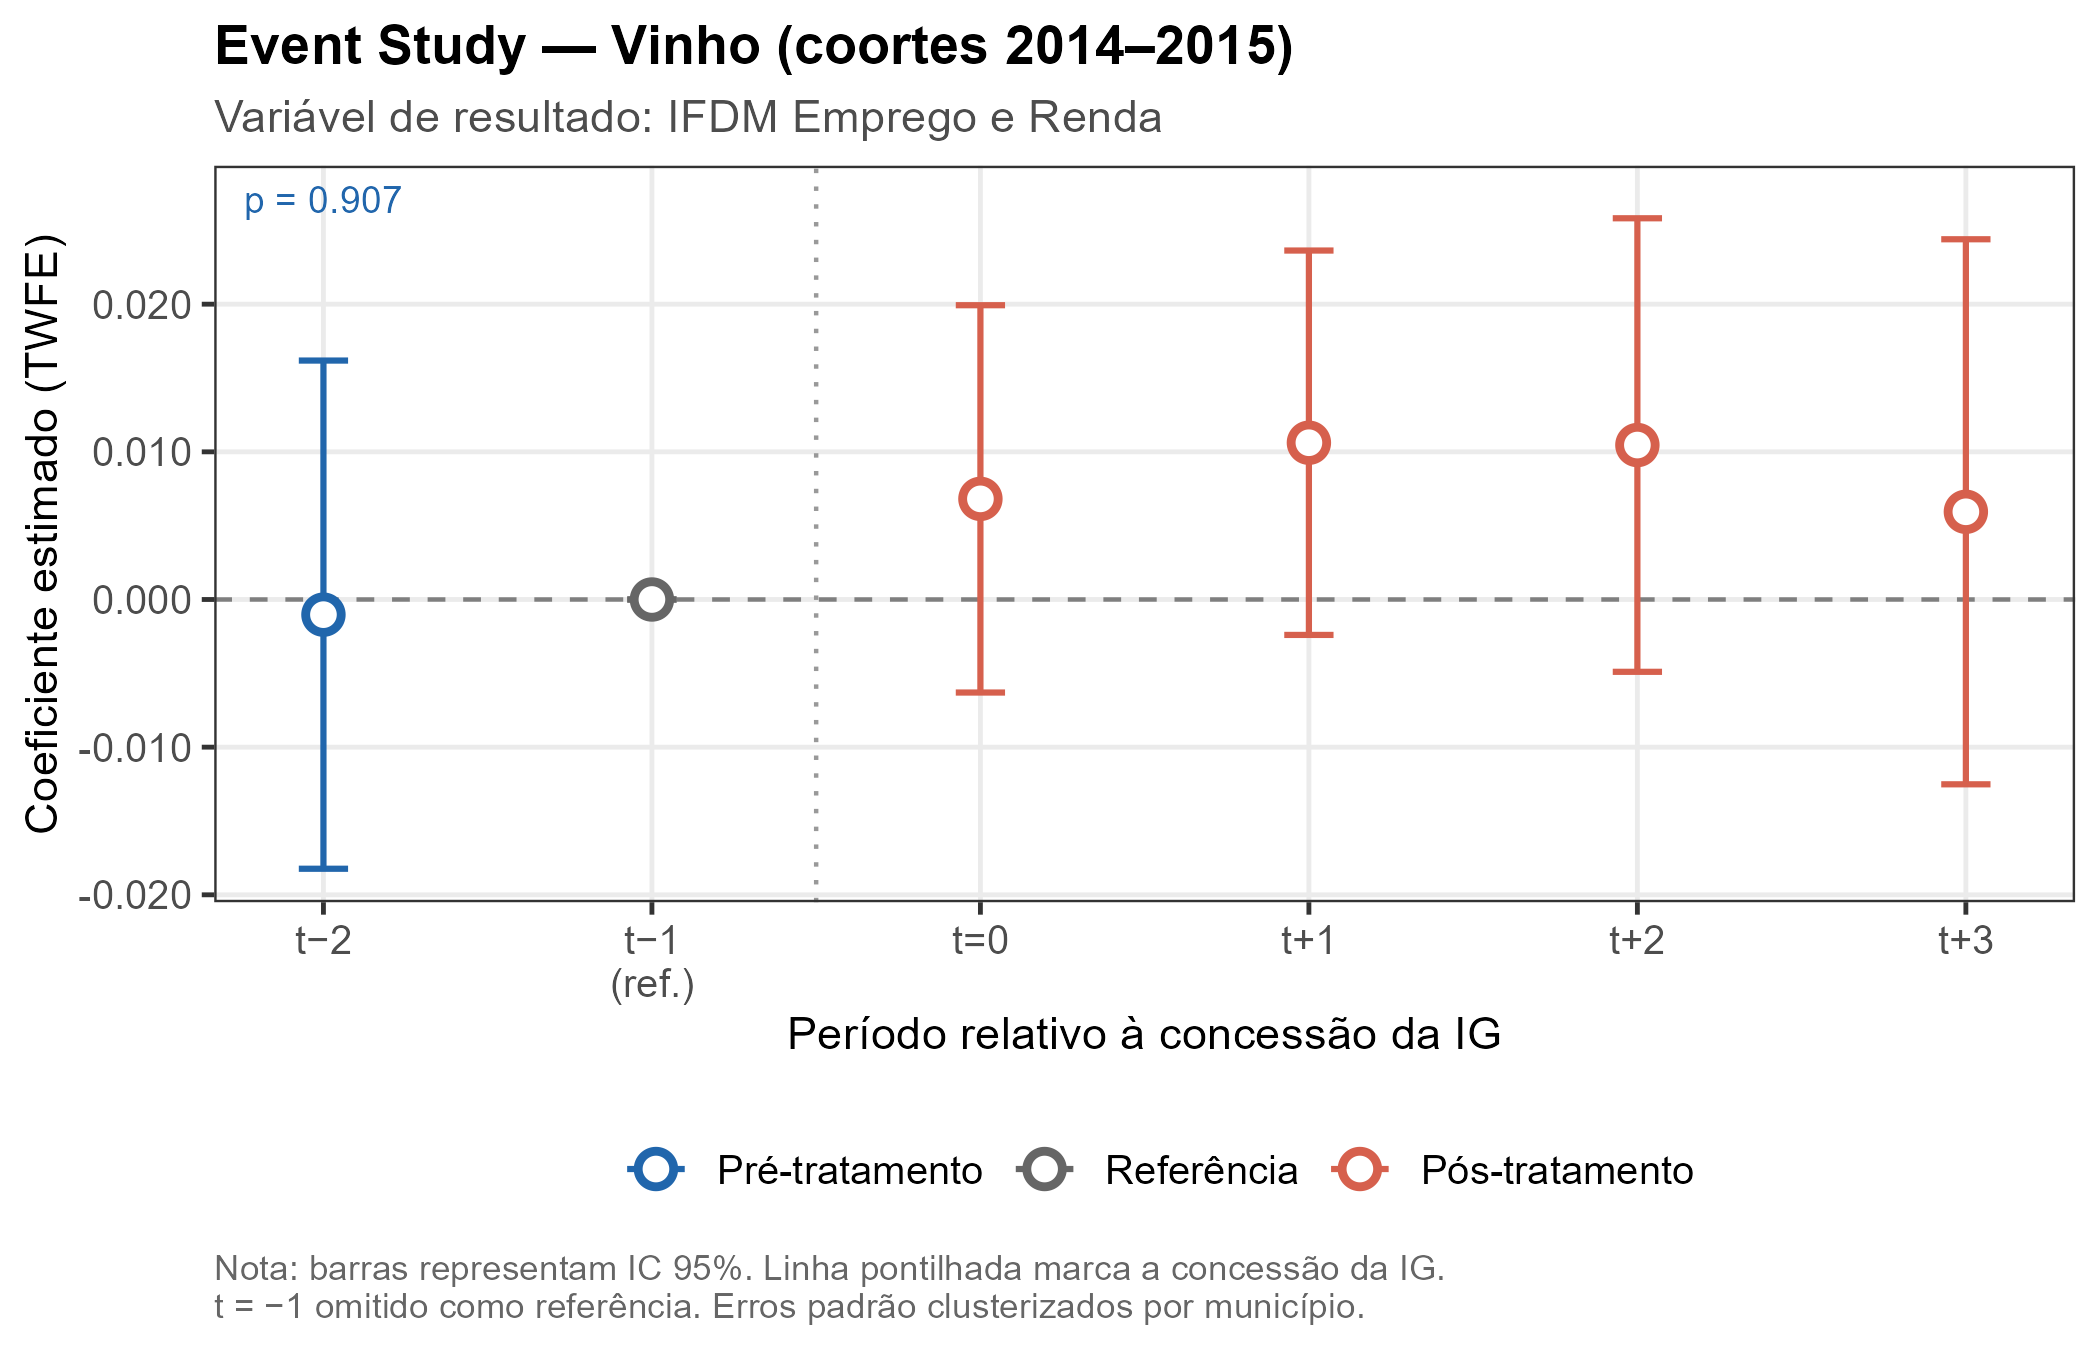
\includegraphics[width=0.82\textwidth]{EventStudy_Vinho.png}
\caption{\textit{Event Study}: Vinho (IFDM Emprego e Renda, coortes 2014-2015)}
\label{fig:es_vinho}
\begin{minipage}{0.85\textwidth}
\small \textit{Nota:} Coeficientes $\hat{\beta}_k$ com IC 95\%. Coeficiente em $t = -2$ não significativo (p = 0,907), validando as tendências paralelas. Ano $-1$ omitido como referência.
\end{minipage}
\end{figure}

\subsection{Síntese Comparativa}

A Tabela~\ref{tab:comparacao} consolida os resultados dos dois produtos e evidencia o contraste entre café e vinho, tanto nos efeitos estimados quanto na validade dos pressupostos de identificação.

\begin{table}[htbp]
\centering
\caption{Comparação dos resultados: café e vinho}
\label{tab:comparacao}
\small
\begin{threeparttable}
\begin{tabular}{lcccc}
\toprule
 & \multicolumn{2}{c}{\textbf{Café}} & \multicolumn{2}{c}{\textbf{Vinho}} \\
\cmidrule(lr){2-3} \cmidrule(lr){4-5}
\textbf{Variável} & PSM ATT & DiD ATT & PSM ATT & DiD ATT \\
\midrule
IFDM Geral            & $+$0,009 (0,58) & $+$0,009 (0,08) & $+$0,020 (0,40) & $+$0,009 (0,21) \\
IFDM Educação         & $+$0,013 (0,40) & $\cdot$         & $-$0,012 (0,65) & $-$0,015 (0,10) \\
IFDM Saúde            & $+$0,018 (0,34) & $\cdot$         & $+$0,035 (0,11) & $+$0,016 (0,34) \\
\textbf{IFDM Emprego} & $+$0,022 (0,41) & $+$0,001 (0,90) & $+$0,038 (0,30) & $\mathbf{+0{,}027^{***}}$ (0,006) \\
\midrule
Tend.\ paralelas & \multicolumn{2}{c}{\textbf{Violadas} ($t{-}2$: p $<$ 0,001)} & \multicolumn{2}{c}{\textbf{Válidas} ($t{-}2$: p = 0,907)} \\
Robustez PSM     & \multicolumn{2}{c}{0/8 significativos} & \multicolumn{2}{c}{$\cdot$} \\
\textbf{Conclusão} & \multicolumn{2}{c}{\textbf{Efeito nulo}} & \multicolumn{2}{c}{\textbf{Emprego: efeito real}} \\
\bottomrule
\end{tabular}
\begin{tablenotes}
\small
\item p-valores entre parênteses. $^{***}$ p $<$ 0,01.
\end{tablenotes}
\end{threeparttable}
\end{table}

Para o café, o pressuposto de tendências paralelas é violado e nenhuma especificação PSM produz efeito significativo, contrariando os resultados de \citet{medeiros2021raiher}, cujo estudo com PSM sem teste de tendências paralelas havia encontrado efeito positivo. Para o vinho, as tendências paralelas são válidas e o DiD identifica efeito positivo e significativo sobre o emprego e renda local, resultado que, ao contrário do café, pode ser interpretado como causal.

% ============================================================
\section{Discussão}
% ============================================================

Os resultados apresentados na seção anterior permitem responder à pergunta de pesquisa com precisão: o registro de uma Indicação Geográfica não gera, por si só, efeitos econômicos mensuráveis nos municípios brasileiros. O efeito existe, mas é condicional às características da cadeia produtiva, manifestando-se de forma significativa apenas no vinho e especificamente na dimensão de emprego e renda.

\subsection{O contraste entre café e vinho à luz da teoria}

O arcabouço teórico proposto por \citet{belletti2017} oferece uma chave interpretativa precisa para esse contraste. Os autores argumentam que os efeitos de uma IG dependem da articulação entre três elementos: viabilidade econômica das empresas da cadeia produtiva, ação coletiva para promoção e controle de qualidade, e preservação dos recursos territoriais que dão identidade ao produto. Os resultados empíricos sugerem que, para o vinho, esses três elementos convergem de forma mais consistente do que para o café.

A cadeia vinícola brasileira apresenta características estruturais que favorecem a conversão da certificação em emprego e renda. A produção de vinho é intensiva em trabalho ao longo de toda a cadeia, do cultivo à vinificação, e está geograficamente concentrada no Rio Grande do Sul, o que facilita a coordenação coletiva entre produtores e a construção de uma identidade territorial reconhecível. Esse perfil é consistente com as observações de \citet{maiorki2015}, que identificaram, para o setor vinícola do sul do Brasil, que os efeitos econômicos da IG tendem a se materializar por meio do turismo e da visibilidade gerada sobre os demais itens da cadeia produtiva local. O efeito positivo sobre o IFDM Emprego e Renda ($+$0,027; p $=$ 0,006) é compatível com a expansão do enoturismo e da demanda por mão de obra nas vinícolas certificadas, efeito semelhante ao documentado por \citet{desimone2024} para as IGs de vinho europeias.

A cadeia cafeeira apresenta um perfil distinto. A produção de café no Brasil é crescentemente mecanizada, especialmente nas regiões onde se concentram as IGs analisadas (Cerrado Mineiro, Chapada Diamantina), o que limita o potencial de encadeamentos locais de emprego. Além disso, os municípios tratados estão dispersos por quatro estados, dificultando a construção de uma identidade territorial coesa e a coordenação coletiva necessária para que a IG gere externalidades positivas. O achado mais relevante, porém, é a violação das tendências paralelas: o coeficiente em $t{-}2$ de $-$0,031 (p $<$ 0,001) indica que os municípios que receberam IGs de café já se encontravam em trajetória de declínio relativo antes da certificação. Isso é consistente com a hipótese de que municípios em dificuldade buscaram a IG como resposta a esse declínio, e não que a IG tenha sido concedida exogenamente. Nesse contexto, o pressuposto de \citet{vaquero2021} de que os efeitos das IGs dependem das condições territoriais preexistentes encontra respaldo empírico direto: onde as condições eram frágeis, a certificação não foi suficiente para reverter a trajetória.

\subsection{Revisão crítica de Medeiros, Raiher e Passador (2021)}

Os resultados deste estudo contrastam diretamente com os de \citet{medeiros2021raiher}, que identificaram efeitos positivos e significativos das IGs de café sobre o IFDM usando PSM em corte transversal. Essa divergência não decorre de diferença de amostra ou de variável de resultado, mas de limitação metodológica inerente ao corte transversal: o PSM controla por diferenças observáveis entre municípios em um único momento, mas não é capaz de verificar se os grupos já divergiam antes do tratamento.

O \textit{Event Study} demonstra que essa divergência pré-existia: municípios com IG de café estavam em declínio relativo antes de receber a certificação, o que faz com que a recuperação posterior apareça como efeito positivo no PSM, quando na verdade trata-se de reversão à média. Sem o teste de tendências paralelas, o efeito positivo encontrado por \citet{medeiros2021raiher} seria a conclusão natural dos dados. Com o teste, ele se revela espúrio. Essa contribuição metodológica dialoga com a agenda de avaliação de impacto de políticas territoriais identificada na revisão de literatura: como apontam \citet{desimone2024} e \citet{crescenzi2022}, os estudos mais robustos verificam explicitamente o pressuposto de identificação antes de interpretar os coeficientes como causais.

\subsection{Implicações para política pública}

Os resultados têm implicações diretas para o desenho de políticas de promoção de IGs no Brasil. A evidência sugere que a certificação de origem não é um instrumento de desenvolvimento territorial de efeito universal: seu impacto depende de condições estruturais da cadeia produtiva que precisam ser avaliadas antes e durante o processo de registro.

Em particular, os resultados indicam que IGs associadas a cadeias intensivas em trabalho, com potencial para encadeamentos locais e agroturismo, e com produtores territorialmente concentrados e organizados coletivamente, têm maior probabilidade de gerar ganhos mensuráveis em emprego e renda. O vinho ilustra esse perfil; o café, ao menos nas regiões e no período analisados, não. Isso não significa que IGs de café sejam ineficazes em todas as dimensões ou contextos, mas que o efeito sobre o desenvolvimento municipal agregado não é captável com as variáveis e o horizonte temporal disponíveis.

Para os formuladores de política, o achado reforça a recomendação de que o registro da IG seja acompanhado de instrumentos complementares de organização coletiva, promoção territorial e qualificação da mão de obra local, especialmente em cadeias menos intensivas em trabalho, onde a certificação, por si só, parece insuficiente para alterar a trajetória de desenvolvimento dos municípios.

\subsection{Limitações}

Este estudo apresenta algumas limitações que devem ser consideradas na interpretação dos resultados. Primeiro, as IGs de vinho concedidas em 2002 (Vale dos Vinhedos) e 2012 (Vales da Uva Goethe), que totalizam 9 municípios, não possuem pré-período observável no painel 2013-2023 e foram excluídas do \textit{Event Study}. Embora seus efeitos sejam absorvidos pelos efeitos fixos no estimador TWFE, não é possível testar formalmente as tendências paralelas para essas unidades, o que representa uma limitação à validade externa dos resultados para coortes anteriores.

Segundo, os dados de exportação do ComexStat registram o município do exportador, que pode não coincidir com o município produtor, o que introduz ruído na análise das variáveis de comércio exterior. Terceiro, o IFDM, embora seja o principal indicador de desenvolvimento municipal disponível para o período, é construído a partir de registros administrativos que podem subestimar atividades informais, especialmente relevantes em cadeias agrícolas. Por fim, o horizonte de análise (até 2023) pode ser insuficiente para captar efeitos de longo prazo das IGs, especialmente nas coortes mais recentes.

% ============================================================
\section{Conclusão}
% ============================================================

Este estudo investigou se o registro de uma Indicação Geográfica gera efeitos econômicos causais nos municípios brasileiros, comparando dois produtos de cadeias produtivas distintas: o café e o vinho. A combinação de PSM, Diferenças em Diferenças com efeitos fixos e \textit{Event Study} permitiu não apenas estimar o efeito médio do tratamento, mas também testar formalmente o pressuposto de tendências paralelas que sustenta a interpretação causal.

Para o café, os resultados são inequívocos: nenhuma das oito especificações do PSM produz efeito significativo, e o \textit{Event Study} revela violação grave das tendências paralelas (coeficiente em $t{-}2$: $-$0,031; p $<$ 0,001). O efeito positivo identificado por \citet{medeiros2021raiher} com PSM em corte transversal reflete, muito provavelmente, reversão à média de municípios que buscaram a certificação em resposta a um declínio preexistente, e não um impacto causal da política.

Para o vinho, o quadro é distinto. O DiD com efeitos fixos identifica efeito positivo e significativo sobre o IFDM Emprego e Renda ($+$0,027; p $=$ 0,006), e o \textit{Event Study} para as coortes de 2014 e 2015 confirma que as tendências paralelas são válidas (coeficiente em $t{-}2$: $-$0,001; p $=$ 0,907). Esse resultado pode ser interpretado como evidência causal de que as IGs de vinho elevaram o emprego e a renda nos municípios certificados, efeito consistente com o papel do enoturismo e da maior intensidade de trabalho nessa cadeia produtiva.

A mensagem metodológica central deste estudo é que o \textit{Event Study} é indispensável para a identificação causal em desenhos de DiD com tratamento escalonado. Sem ele, a associação positiva encontrada pelo PSM para o café seria interpretada como efeito da política, quando na verdade reflete seleção preexistente. Essa contribuição dialoga com os estudos mais recentes da literatura internacional, que têm incorporado sistematicamente testes de tendências paralelas como condição para interpretação causal \citep{desimone2024, crescenzi2022}.

Do ponto de vista substantivo, os resultados sugerem que a eficácia das IGs como instrumento de desenvolvimento territorial é condicionada às características estruturais da cadeia produtiva. Cadeias intensivas em trabalho, territorialmente concentradas e com potencial para encadeamentos locais tendem a converter a certificação em ganhos mensuráveis de emprego e renda. Cadeias mais mecanizadas e dispersas, como a do café nas regiões analisadas, não apresentam esse padrão.

Como agenda futura, sugere-se: (i) ampliar a análise para outros produtos com IGs no Brasil, como cachaça, queijo e produtos artesanais; (ii) empregar dados da RAIS desagregados por setor para identificar os mecanismos específicos de geração de emprego; (iii) investigar heterogeneidades por tipo de IG (Indicação de Procedência versus Denominação de Origem), dado que a DO exige maior coordenação coletiva e pode gerar efeitos distintos; e (iv) ampliar o horizonte temporal à medida que novos dados do IFDM se tornem disponíveis, permitindo avaliar efeitos de mais longo prazo das coortes recentes.

% ============================================================
\bibliography{referencias}

% ============================================================
\appendix
\section{Scripts de Replicação}

Todas as análises foram realizadas em R 4.2.3. Os scripts estão organizados na seguinte ordem:

\begin{enumerate}
  \item \texttt{01\_integrar\_dados\_cafe.R} - Integração MAPA, IFDM e PIB
  \item \texttt{02\_PSM\_cafe.R} - PSM \textit{baseline} (IFDM)
  \item \texttt{02\_PSM\_cafe\_economicas.R} - PSM variáveis econômicas
  \item \texttt{03\_Robustez\_PSM\_cafe\_v2.R} - 8 testes de robustez
  \item \texttt{05\_DiD\_Preciso\_cafe.R} - DiD com anos exatos (IFDM)
  \item \texttt{06\_DiD\_Economicas\_FINAL.R} - DiD variáveis econômicas
  \item \texttt{09\_Vinho\_Mapeamento.R} - Identificação dos municípios de vinho
  \item \texttt{10\_Exportacoes\_PSM\_DiD.R} - PSM e DiD exportações café
  \item \texttt{11\_Vinho\_PSM\_DiD.R} - PSM, DiD e Event Study vinho
\end{enumerate}

\end{document}
